% NH-1: A Vitality-Driven, Learning-Adaptive Distributed Hash Table
% Author: David A. Smith, YZ.social
% Target: 12-page two-column conference format (IEEE P2P / ICDCS / NSDI workshop)
%
% Build:  tectonic nh1-paper.tex
% Or:     pdflatex nh1-paper && bibtex nh1-paper && pdflatex nh1-paper && pdflatex nh1-paper

\documentclass[conference]{IEEEtran}
\IEEEoverridecommandlockouts

% ── Packages ─────────────────────────────────────────────────────────────────
\usepackage{cite}
\usepackage{amsmath,amssymb}
\usepackage{algorithmic}
\usepackage{graphicx}
\usepackage{textcomp}
\usepackage{xcolor}
\usepackage{booktabs}
\usepackage{url}
\usepackage{tikz}
\usetikzlibrary{positioning, arrows.meta, shapes.geometric, fit, backgrounds}
\usepackage{pgfplots}
\pgfplotsset{compat=1.18}
\usepackage{hyperref}
\hypersetup{colorlinks=true, linkcolor=black, citecolor=black, urlcolor=blue}

% ── Custom commands ──────────────────────────────────────────────────────────
\newcommand{\nhone}{NH-1\xspace}
\usepackage{xspace}
\newcommand{\NDHT}{N-DHT\xspace}
\newcommand{\KDHT}{K-DHT\xspace}
\newcommand{\GDHT}{G-DHT\xspace}
\newcommand{\NXseventeen}{NX-17\xspace}

% ── Title and authors ────────────────────────────────────────────────────────
\title{N-DHT: A Learning-Adaptive Distributed Hash Table\\and Axonal Publish/Subscribe\\[0.3em]{\normalsize\normalfont v0.3.51 \quad 2026-05-16}}

\author{
\IEEEauthorblockN{David A. Smith}
\IEEEauthorblockA{YZ.social\\
\texttt{davidasmith@gmail.com}}
}

\begin{document}
\maketitle
% IEEE conference style suppresses page numbers by default
% (\pagestyle{empty}). Override after \maketitle so reviewers can
% reference page numbers in comments.
\pagestyle{plain}
\thispagestyle{plain}

% ─────────────────────────────────────────────────────────────────────────────
\begin{abstract}
Distributed hash tables (DHTs) are the substrate of content-addressable
peer-to-peer systems, but the canonical Kademlia design routes messages in
$O(\log N)$ hops without regard to network locality, yielding multi-second
tail latency on million-node networks. We present two contributions.
First, the \emph{Geographic DHT} (\GDHT) embeds an S2 cell prefix in
node identifiers so that XOR distance in ID space approximates physical
distance --- a simple structural change that reduces $500$\,km regional
lookup latency by $3.4\times$ over Kademlia at $25\,000$ nodes. Second,
\nhone is a learning-adaptive DHT layered above the Kademlia/\GDHT
substrate that introduces \emph{vitality} --- a per-edge score
$\mathrm{weight} \times \mathrm{recency}$ in which the weight is
reinforced by successful traffic (Hebbian long-term potentiation) and
recency exponentially decays after a synaptic-tagging-style protection
window. A single vitality-based admission gate replaces five distinct
mechanisms in the predecessor \NXseventeen, consolidating eighteen
specialized rules and forty-four parameters into twelve each. On a
$50\,000$-node simulator, \NXseventeen routes at $1.18\times$ the Dabek
$3\delta$ analytical floor~\cite{dabek2004designing} --- within $36$\,ms
of the analytical lower bound for any recursive $O(\log N)$ DHT --- and
\nhone plateaus at $1.28\times$. \nhone provides built-in publish/subscribe
via axonal delivery trees, achieving 100\% baseline and 100\% recovered
delivery under $5\%$ churn, and recovers from single-bridge network
partitions through cooperative re-stitching driven by hop caching and
triadic closure. An ablation that strips the \GDHT prefix shows learning
alone outperforms Kademlia by $26\%$, demonstrating that the
contribution is structural rather than a consequence of locality
engineering.
\end{abstract}

% ═════════════════════════════════════════════════════════════════════════════
\section{Introduction}
\label{sec:intro}

Peer-to-peer applications --- file sharing, blockchain peer discovery, content
addressing, decentralized identity, censorship-resistant messaging --- depend
on a name resolution substrate that no single party controls. The canonical
answer for two decades has been the distributed hash
table~\cite{stoica2001chord,maymounkov2002kademlia,rowstron2001pastry,zhao2004tapestry,ratnasamy2001can},
which assigns every key and every node an address in a shared identifier
space, then routes messages from a key to its responsible node in
$O(\log N)$ hops. Kademlia~\cite{maymounkov2002kademlia}, the dominant
production deployment (BitTorrent Mainline, Ethereum devp2p, IPFS, Tor v3
hidden services), uses an XOR distance metric over $160$-bit identifiers and
provably halves the distance to the destination on every hop.

\emph{Hop count, however, is not latency.} Random identifiers spread peers
homogeneously across the globe; the average pair sits roughly half the planet
apart, with about $100$\,ms one-way round-trip time. With $N = 10^6$ nodes,
$\log_2 N \approx 20$, and the naive estimate gives an average message time
of $20 \times 100 = 2$\,seconds. For real-time applications --- pub/sub,
voice, gaming, live coordination --- this is unacceptable. The latency
problem is the dominant practical barrier between DHT theory and DHT
deployment.

\paragraph{Locality is necessary but not sufficient.}
The first generation of latency-aware DHTs put network proximity in the
routing layer itself. Pastry~\cite{rowstron2001pastry} maintains a three-tier
routing state (a prefix-matched routing table $R$, a numerically-closest leaf
set $L$, and an RTT-closest neighborhood set $M$), populating each table
slot with the closest node by RTT among candidates with the appropriate
prefix. Tapestry~\cite{zhao2004tapestry} pushes the same instinct further,
storing soft-state location pointers along the publish path and recovering
the closest replica via path intersection. Coral~\cite{freedman2004coral}
relaxes the strict-DHT promise and builds nested RTT clusters explicitly.
Vivaldi~\cite{dabek2004vivaldi} synthesizes per-node Euclidean coordinates
that predict pair-wise RTT without active probing.

These designs reduce the per-hop constant. They do not, however,
\emph{learn} from the traffic that flows through them. A Pastry routing
table is set at insertion time and refreshed lazily. A Coral cluster
hierarchy is determined by RTT thresholds, not by which paths are
actually used. Vivaldi predicts latency but does not act on those
predictions in routing without a separate decision layer. The frontier
is a routing fabric whose composition adapts to observed traffic ---
where \emph{which peers are kept} is a function of which paths the network
actually carries.

\paragraph{The analytical floor.} Dabek \emph{et~al.}~\cite{dabek2004designing}
proved that for any recursive $O(\log N)$ DHT, total lookup latency
converges to a hard analytical floor:
\begin{equation}
\text{lookup ms} \approx \delta + \frac{\delta}{2} + \frac{\delta}{4} + \cdots = 3\delta
\label{eq:dabek}
\end{equation}
where $\delta$ is the median pairwise one-way internet latency. Each
successive lookup hop covers a geometrically halving fraction of the
remaining ID-space, so the second-to-last hop is half the cost of the
last, the third-to-last a quarter, and so on. The series converges
regardless of $N$. Even an oracle that always picks the lowest-RTT
finger cannot beat this bound. Until now, no published DHT has been
measured \emph{at} this floor.

\paragraph{Contributions.}
This paper presents two protocol contributions and three empirical results
that together establish a new operating point for the DHT design space:

\begin{enumerate}
\item \textbf{The Geographic DHT (\GDHT).} A simple structural extension
of Kademlia: the top $8$ bits of every node identifier encode the S2
cell of the node's claimed geographic position. With this prefix, XOR
distance in identifier space approximates physical distance, and a
node's bootstrap routing table is biased toward local peers without
any change to the routing algorithm itself. \GDHT reduces $500$\,km
regional lookup latency by $3.4\times$ over Kademlia at $25\,000$
nodes (\S\ref{sec:gdht}), and is the substrate on which \nhone's
learning is layered.

\item \textbf{\nhone}, a learning-adaptive DHT layered above the
Kademlia/\GDHT substrate, that consolidates the $18$-rule, $44$-parameter
\NXseventeen lineage into a $12$-rule, $12$-parameter protocol
governed by a single vitality-based admission gate (\S\ref{sec:nh1}).
The consolidation is a direct application of Hebbian long-term
potentiation~\cite{hebb1949organization,bliss1973long}: every
successful lookup reinforces the synaptic weights along the traversed
path, every unused edge decays over time, and the routing table
evolves toward a traffic-shaped optimum.

\item \textbf{First measurement of an $O(\log N)$ DHT at the Dabek
$3\delta$ analytical floor.} \NXseventeen plateaus within $1.18\times$
the floor at $25\,000$ and $50\,000$ nodes; \nhone plateaus at
$1.28\times$. Kademlia worsens from $2.01\times$ to $2.65\times$ over
the same range (\S\ref{sec:eval-floor}).

\item \textbf{Axonal publish/subscribe}, a built-in delivery primitive
structurally equivalent to SCRIBE~\cite{castro2002scribe} but adaptive
under churn. \nhone achieves $100\%$ baseline delivery and $100\%$
recovered delivery at $5\%$ churn through routed re-subscribe alone ---
no replication, no gossip, no parent tracking (\S\ref{sec:pubsub}).

\item \textbf{Geography ablation.} Stripping the \GDHT prefix and
re-running the comparison shows that with \emph{no} geographic
structure, \NXseventeen still routes $26\%$ faster than Kademlia and
\nhone routes $8\%$ faster (\S\ref{sec:eval-geo}). Learning is doing
real work, not sharpening pre-existing geographic structure.
\end{enumerate}

\noindent
The contributions rest on a publicly available, open-source simulator
($\sim\!25\,000$ lines of JavaScript) whose every CSV is in the
repository~\cite{dhtsim2026}.

\paragraph{Roadmap.}
\S\ref{sec:related} surveys the lineage and related work. \S\ref{sec:substrate}
presents the neuromorphic substrate --- the biology of long-term
potentiation and its precise mapping into routing-table mechanics.
\S\ref{sec:nh1} describes \nhone's five operations, twelve rules, and
vitality function in detail. \S\ref{sec:pubsub} covers axonal pub/sub.
\S\ref{sec:gdht} covers the geographic prefix used as a bootstrap seed.
\S\ref{sec:eval} reports the four headline results. \S\ref{sec:discussion}
discusses limitations, including a third-party red-team analysis identifying
deploy blockers~\cite{nh1redteam2026}. \S\ref{sec:future} sketches future
work, and \S\ref{sec:conclusion} concludes.

% ═════════════════════════════════════════════════════════════════════════════
\section{Background and Related Work}
\label{sec:related}

\paragraph{The Berkeley/Cambridge DHT lineage.}
\nhone inherits structurally from three foundational designs. Kademlia
\cite{maymounkov2002kademlia} provides the substrate: $160$-bit random
identifiers, a symmetric XOR distance metric (which makes routing
self-organizing because every incoming or outgoing message updates a
$k$-bucket), $K=20$ peers per stratum, and $\alpha$-parallel asynchronous
\textsc{find\_node} queries. Kademlia's empirical observation that old
peers are more reliable than new peers~\cite{saroiu2003measurement}
becomes \nhone's vitality recency multiplier. Pastry~\cite{rowstron2001pastry}
contributes
the three-tier routing state ($R$, $L$, $M$), the locality-preserving
join algorithm in which a new node $X$ takes row $n$ of its routing
table from the $n$-th node along its routed-join path, and SCRIBE
\cite{castro2002scribe}, the structural ancestor of axonal pub/sub.
Tapestry~\cite{zhao2004tapestry} contributes the locality-aware
routing table (closest node by RTT per slot, built at insertion),
soft-state location pointers along publish paths, and surrogate
routing (when the deterministic root is dead, route to the closest
live identifier). \nhone retains all of these mechanisms in some form;
the contribution is to make them \emph{learn} from observed traffic.

\paragraph{Latency analysis.}
Dabek \emph{et~al.}~\cite{dabek2004designing} (NSDI 2004) prove the $3\delta$
floor for any recursive $O(\log N)$ DHT and show DHash++ approaches it
through proximity neighbor selection, server selection over erasure-coded
fragments, and the integration of routing and fetching. Tapestry's
companion measurement~\cite{zhao2004tapestry} reports a complementary
metric --- relative delay penalty (RDP) --- with median wide-area RDP
near $1$ and $90$th-percentile near $2$--$3$. These analyses set the
methodological standard for DHT-latency reporting and the
target~\nhone aims to match.

\paragraph{Adaptive maintenance.}
A recurring instinct in the post-2003 DHT literature is that routing-table
maintenance should adapt to observed conditions rather than run on a
fixed schedule. Mahajan, Castro, and Rowstron~\cite{mahajan2003controlling}
introduce a cost-of-reliability framework. Krishnamurthy
\emph{et~al.}~\cite{krishnamurthy2005statistical} model Chord under Poisson
churn analytically. Ghinita and Teo~\cite{ghinita2006adaptive} present
the closest existing match in mechanism family to \nhone: each peer
estimates local node-failure rate $\mu$, join rate $\lambda$, and
network size $N$; computes pointer-staleness probabilities; and
triggers cheap liveness checks or expensive accuracy checks only when
warranted. Their headline --- $3.4\times$ lower lookup failure at
$2.4\times$ lower communication overhead under variable churn ---
demonstrates that self-tuning works. \nhone applies the same instinct
to a different observable: not maintenance rate but routing-table
\emph{composition}.

\paragraph{Resilience and load.}
Castro \emph{et~al.}~\cite{castro2002secure} prove the foundational triplet
for Byzantine resistance: constrained routing tables, secure node-ID
assignment, and redundant routing. Harvesf and
Blough~\cite{harvesf2007design} make the redundant-routing piece
concrete with MaxDisjoint replica placement, achieving $90\%$ lookup
success at $50\%$ malicious nodes. Makris
\emph{et~al.}~\cite{makris2017novel} address the orthogonal problem of
Zipf-distributed request rates with the Directory For Exceptions
mechanism --- a hybrid of consistent hashing~\cite{karger1997consistent}
and a small distributed
override that migrates hot keys to less-loaded peers. \nhone~\S\ref{sec:future}
identifies these as the canonical mitigations for two open security
and load-balancing gaps.

\paragraph{Locality alternatives.}
Beyond Pastry/Tapestry's structural locality, two adaptive alternatives
warrant comparison. Coral~\cite{freedman2004coral} builds nested clusters
at increasing RTT thresholds, relaxing the strict DHT promise (sloppy
hashing) to deliver content-distribution at scale.
Vivaldi~\cite{dabek2004vivaldi} computes synthetic per-node coordinates
that predict pair-wise RTT to peers a node has never directly contacted.
Both treat the network as something to measure and adapt to. \nhone
goes further: rather than measure or predict, it learns paths
themselves through reinforcement on the routing layer.

% ═════════════════════════════════════════════════════════════════════════════
\section{The Neuromorphic Substrate}
\label{sec:substrate}

The framing of \nhone as ``neuromorphic'' is not decorative. The brain
and a peer-to-peer DHT face a precisely shared engineering problem,
and the solution that biological evolution found applies to
overlay routing with no metaphorical slippage.

\paragraph{The shared engineering problem.}
A single neuron carries on the order of $10^4$ synapses --- a hard upper
bound set by the energetic cost of maintaining synaptic
machinery~\cite{laughlin2003communication}. The number of \emph{candidate}
synaptic partners --- other neurons whose axons could reach it --- is
orders of magnitude larger. The neuron cannot store every co-firing event;
it must score, prioritize, and prune. A peer-to-peer node in a browser
deployment is bounded by WebRTC's connection limit (typically $50$--$200$
peers, with Safari at $\sim\!95$). The number of candidate peers in a
$50\,000$-node overlay is three orders of magnitude larger. The same
storage-constrained, more-candidates-than-capacity problem appears in
both systems. \emph{The biological solution is the engineering solution.}

\paragraph{Long-term potentiation.}
The mechanism by which the brain remembers which paths are useful is
\emph{long-term potentiation} (LTP), discovered by Bliss and
L\o{}mo~\cite{bliss1973long} in rabbit hippocampus. A few high-frequency
electrical bursts to the perforant path produced post-synaptic responses
that remained elevated for \emph{weeks}. The molecular cascade that
underlies LTP gives the brain a coincidence-aware, durable, and
selectively reversible learning signal:

\begin{itemize}
\item \emph{NMDA receptors as coincidence detectors.} Glutamate from the
pre-synaptic neuron only opens NMDA channels if the post-synaptic
neuron is \emph{already} depolarized. The signal is ``I fired and you
fired,'' not just ``I fired.''
\item \emph{Calcium-mediated AMPA insertion.} Calcium influx through
opened NMDA channels triggers insertion of additional AMPA receptors
into the post-synaptic membrane. The synapse is now physically more
sensitive to subsequent glutamate release.
\item \emph{Consolidation.} Within roughly $30$ minutes, gene
transcription and new protein synthesis produce a durable physical
change. Sometimes new dendritic spines form. The synapse is
re-weighted permanently~\cite{bear2020neuroscience}.
\end{itemize}

\noindent
The opposing process, long-term depression (LTD), weakens synapses
under low-frequency stimulation~\cite{stanton1989associative}. LTP and
LTD together let the brain \emph{learn} which routes among neurons are
worth keeping.

\paragraph{Synaptic tagging and capture.}
Frey and Morris~\cite{frey1997synaptic} added a critical refinement:
recently potentiated synapses carry a transient ``tag'' that protects
them from being overwritten by competing potentiation events, but only
for a brief consolidation window. The tag bridges the timescale gap
between the coincidence detection (milliseconds) and the protein
synthesis that consolidates the change (tens of minutes). Without it,
learning would be self-destructive: the very synapses just discovered
to be useful would be the most likely to be overwritten by the next
high-frequency event. \nhone's \texttt{INERTIA\_DURATION} parameter
implements precisely this protection in routing.

\paragraph{The Hebbian rule.}
Donald Hebb's 1949 formulation~\cite{hebb1949organization} predates
the molecular discoveries by two decades and remains the cleanest
abstraction:

\begin{quote}
\emph{Neurons that fire together, wire together.}
\end{quote}

\noindent
Every weight in every artificial neural network ultimately invokes
this rule. \nhone applies it not to perception but to \emph{routing}:
peers that successfully carry traffic together earn higher weights;
peers that carry no traffic decay. The routing table is shaped by
the queries it serves, in exactly the way a cortical region's
synaptic structure is shaped by the sensory input it processes.

\paragraph{Mapping table.}
The translation from neuroscience mechanisms to \nhone source-code
mechanisms is direct, not analogical (Figure~\ref{fig:mapping},
Table~\ref{tab:mapping}). Every term has one corresponding artifact
in the codebase.

\begin{figure}[t]
\centering
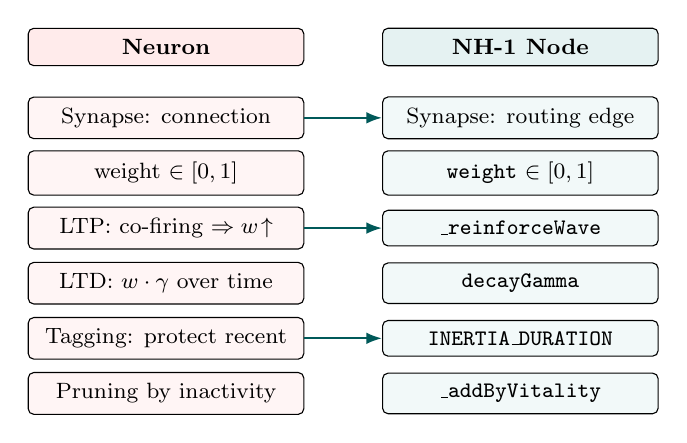
\begin{tikzpicture}[
  every node/.style={font=\footnotesize},
  bx/.style={draw, rounded corners=2pt, minimum width=3.5cm, align=center, inner sep=4pt},
  hd/.style={font=\footnotesize\bfseries},
  ar/.style={-{Latex[length=2mm]}, thick, color=teal!70!black},
]
% Left column - Neuron
\node[bx, fill=red!8] (neuron) at (0,3.0) {\textbf{Neuron}};
\node[bx, fill=red!4] (s1) at (0,2.1) {Synapse: connection};
\node[bx, fill=red!4] (s2) at (0,1.4) {weight $\in [0,1]$};
\node[bx, fill=red!4] (s3) at (0,0.7) {LTP: co-firing $\Rightarrow w\!\uparrow$};
\node[bx, fill=red!4] (s4) at (0,0.0) {LTD: $w \cdot \gamma$ over time};
\node[bx, fill=red!4] (s5) at (0,-0.7) {Tagging: protect recent};
\node[bx, fill=red!4] (s6) at (0,-1.4) {Pruning by inactivity};

% Right column - NH-1
\node[bx, fill=teal!10] (dht) at (4.5,3.0) {\textbf{NH-1 Node}};
\node[bx, fill=teal!5] (n1) at (4.5,2.1) {Synapse: routing edge};
\node[bx, fill=teal!5] (n2) at (4.5,1.4) {\texttt{weight} $\in [0,1]$};
\node[bx, fill=teal!5] (n3) at (4.5,0.7) {\texttt{\_reinforceWave}};
\node[bx, fill=teal!5] (n4) at (4.5,0.0) {\texttt{decayGamma}};
\node[bx, fill=teal!5] (n5) at (4.5,-0.7) {\texttt{INERTIA\_DURATION}};
\node[bx, fill=teal!5] (n6) at (4.5,-1.4) {\texttt{\_addByVitality}};

% Mapping arrows (one between each pair, not shown for visual cleanliness on every row)
\draw[ar] (s1) -- (n1);
\draw[ar] (s3) -- (n3);
\draw[ar] (s5) -- (n5);
\end{tikzpicture}
\caption{Direct correspondence between neuromorphic mechanisms (left)
and \nhone routing-table operations (right). Every term on the right
has one corresponding artifact in the codebase. Arrows are shown on a
representative subset to avoid visual clutter; the full mapping is in
Table~\ref{tab:mapping}.}
\label{fig:mapping}
\end{figure}

\begin{table}[t]
\centering
\caption{Direct mapping from biological mechanisms to \nhone routing-table operations.}
\label{tab:mapping}
\small
\begin{tabular}{@{}p{0.42\columnwidth}p{0.50\columnwidth}@{}}
\toprule
\textbf{Neuroscience} & \textbf{\nhone} \\
\midrule
Synapse --- a connection between neurons & A peer entry in the routing table (\texttt{Synapse} class) \\
Synaptic weight --- readiness to fire & \texttt{weight} $\in [0,1]$ \\
LTP --- co-firing strengthens the connection & Successful lookup increments weights along the traversed edges (\texttt{\_reinforceWave}) \\
LTD --- disuse weakens & Time-based decay each tick (\texttt{weight *= decayGamma}) \\
NMDA coincidence detection & Weight increments only on successful traffic, not every probe \\
Synaptic tagging~\cite{frey1997synaptic} & \texttt{inertiaDuration} epochs prevent eviction of recently reinforced synapses \\
Pruning of unused connections & \texttt{\_addByVitality} evicts the lowest-vitality (\texttt{weight}~$\times$~\texttt{recency}) edge \\
\bottomrule
\end{tabular}
\end{table}

\paragraph{Looking forward: metaplasticity.}
The classical Hebbian story says synapses change in response to
activity. Bienenstock, Cooper, and Munro~\cite{bcm1982theory} proposed
that the threshold separating LTP from LTD is itself an adaptive
variable, sliding based on the post-synaptic neuron's recent average
activity. This is \emph{metaplasticity} --- plasticity of plasticity ---
and it produces homeostatic self-balancing toward a target activity
level rather than runaway potentiation or silence. \nhone's parameters
are presently fixed constants chosen by sweep. A metaplastic \nhone,
in which \texttt{decayGamma}, \texttt{INERTIA\_DURATION}, and the
annealing schedule are themselves observation-driven, is the natural
next step (\S\ref{sec:future}).

% ═════════════════════════════════════════════════════════════════════════════
\section{\nhone Architecture}
\label{sec:nh1}

\nhone is a learning-adaptive DHT layered above an unmodified Kademlia
substrate. The contribution sits between Kademlia's $k$-buckets and the
application: every routing decision, every bucket admission, every churn
response runs through a single vitality function. This section walks the
architecture in five operations, presents the unified admission gate that
replaces five distinct mechanisms in the predecessor \NXseventeen, and
gives end-to-end pseudocode for one lookup.

\subsection{Five operations, one vitality model}
\label{sec:nh1-overview}

Every \nhone behavior decomposes into one of five operations:

\begin{itemize}
\item \textbf{NAVIGATE} --- choose a next hop given a target.
\item \textbf{LEARN} --- reinforce edges that carried successful traffic.
\item \textbf{FORGET} --- decay unused edges; evict by vitality.
\item \textbf{EXPLORE} --- inject controlled randomness to escape local minima.
\item \textbf{STRUCTURE} --- bootstrap and steady-state topology maintenance.
\end{itemize}

\noindent
Twelve rules implement these operations (Table~\ref{tab:rules}); twelve
parameters tune them (Table~\ref{tab:params}). Every rule is grounded in
either the neuromorphic substrate (\S\ref{sec:substrate}) or the foundational
DHT literature (\S\ref{sec:related}); none was added speculatively.

\begin{table}[t]
\centering
\caption{The twelve rules of \nhone, organized by operation.}
\label{tab:rules}
\small
\begin{tabular}{@{}cp{0.40\columnwidth}p{0.30\columnwidth}@{}}
\toprule
\textbf{\#} & \textbf{Rule} & \textbf{Operation} \\
\midrule
1 & Stratified bootstrap & \textsc{structure} \\
2 & Mixed-capacity (highway\%) deployment & \textsc{structure} \\
3 & Action-Potential (AP) routing & \textsc{navigate} \\
4 & Two-hop lookahead & \textsc{navigate} \\
5 & Iterative fallback (= surrogate routing) & \textsc{navigate} \\
6 & Long-Term Potentiation (LTP) & \textsc{learn} \\
7 & Triadic closure & \textsc{learn} \\
8 & Hop caching + lateral spread & \textsc{learn} \\
9 & Incoming promotion & \textsc{learn} \\
10 & Vitality-based eviction & \textsc{forget} \\
11 & Temperature annealing + reheat & \textsc{explore} \\
12 & Epsilon-greedy first hop & \textsc{explore} \\
\bottomrule
\end{tabular}
\end{table}

\subsection{The vitality function}
\label{sec:nh1-vitality}

Every synapse $s$ carries two scalars: a learned weight $w_s \in [0,1]$ and a
last-reinforcement epoch $t_s$. The vitality function combines them
multiplicatively:
\begin{equation}
\mathrm{vitality}(s) = w_s \times \mathrm{recency}(s)
\label{eq:vitality}
\end{equation}
\begin{equation}
\mathrm{recency}(s) =
\begin{cases}
1.0 & \text{if } t - t_s < I \\
e^{-(t - t_s - I)/\tau_r} & \text{otherwise}
\end{cases}
\label{eq:recency}
\end{equation}
where $t$ is the current epoch (lookup count), $I$ is the
\texttt{INERTIA\_DURATION} (default $20$), and $\tau_r$ is the
\texttt{RECENCY\_HALF\_LIFE} ($50$). The piecewise definition implements
synaptic tagging~\cite{frey1997synaptic}: a freshly reinforced synapse is
locked at full recency for $I$ epochs --- it cannot be evicted regardless of
vitality competition --- after which recency decays exponentially. Without
this lock, learning would be self-destructive: the routing table would
discard the very edges it just discovered to be useful.

The weight itself is updated on two events. On every successful lookup
(LTP, Rule~6), each synapse $s$ on the traversed path gains $w_s
\leftarrow \min(1, w_s + \eta)$ for $\eta = 0.05$. On every tick of the
decay clock, every synapse loses $w_s \leftarrow \gamma \cdot w_s$ for
$\gamma = 0.995$. A synapse with $w_s$ near $1$ that is then unused for
$\sim\!100$ ticks decays to $\sim\!0.6$; combined with the recency
exponential, its vitality drops below the typical eviction threshold
within $\sim\!200$ unused lookups. Frequently used edges accumulate
weight faster than decay erodes it; unused edges fade.

\subsection{The synaptome}
\label{sec:nh1-synaptome}

The bounded, vitality-scored set of outgoing edges at a node is the
\emph{synaptome}, capped at $50$ entries (a safe cross-browser WebRTC
target; Safari measured at $\sim\!95$ peak connections). The synaptome is
\nhone's analog of Pastry's three-tier routing
state~\cite{rowstron2001pastry} (routing table $R$, leaf set $L$,
neighborhood set $M$) consolidated into a single tier scored by vitality.
The roles persist in latent form:

\begin{itemize}
\item \emph{High-vitality entries} (recently reinforced, locked) play the
leaf-set role: well-trafficked nearby peers, dominate terminal-hop routing.
\item \emph{Mid-vitality entries} cover XOR strata in the manner of
Pastry's $R$: ensures every distance band has a candidate.
\item \emph{Low-vitality entries plus a 2-hop neighborhood sample} play the
$M$ role: candidates for annealing replacement, kept warm but not routed
through.
\end{itemize}

\noindent
A reader familiar with Pastry can think of the synaptome as Pastry's three
tables collapsed into a single vitality-scored set. The bookkeeping is
unified; the structural roles are unchanged.

\subsection{NAVIGATE: Action-Potential routing}
\label{sec:nh1-navigate}

Each lookup hop scores synapses by the Action-Potential metric (Rule~3):
\begin{equation}
\mathrm{AP}(s, k) = \mathrm{progress}(s, k) \times w_s \times \tfrac{1}{2}^{(\ell_s / 100)}
\label{eq:ap}
\end{equation}
where $\mathrm{progress}(s, k) = d(\mathrm{self}, k) - d(s.\mathrm{peer}, k)$
is the XOR-distance reduction toward target $k$, $w_s$ is the learned
weight, and $\ell_s$ is the observed round-trip latency in milliseconds.
The latency penalty halves AP every $100$\,ms, making nearby fast peers
preferred over slightly-better-XOR distant ones. AP routing is therefore
\emph{latency-aware} rather than purely \emph{distance-aware}: it inherits
the locality property that defines Pastry and Tapestry, but evaluates it
\emph{dynamically per lookup} from observed RTT rather than statically at
insertion.

\paragraph{Two-hop lookahead (Rule~4).}
When the top-$\alpha$ AP scores are bunched (no decisive first hop),
\nhone probes the top $\alpha = 2$ first hops for \emph{their} best
second hops and picks the path with the highest combined
$\mathrm{AP}(\mathrm{first}) \times \mathrm{AP}(\mathrm{second})$. The
lookahead is exactly two hops --- never three --- so each step is
locally optimal across two hops while compute remains bounded at
$O(\alpha \cdot |\mathrm{synaptome}|)$ per step.

\paragraph{Iterative fallback (Rule~5).}
When AP returns no candidate --- every neighbor has $\mathrm{progress} \le 0$,
i.e.\ would move \emph{away} from the target --- \nhone falls back to
$k$-closest-from-synaptome regardless of progress. This rescues lookups
that would otherwise stall in dead corridors. The mechanism is \emph{surrogate
routing} in Tapestry's terminology~\cite{zhao2004tapestry}: when the
deterministic next-hop cannot be served, route to the closest live
identifier. We adopt the canonical term to make the lineage explicit.

\subsection{LEARN: four reinforcement mechanisms}
\label{sec:nh1-learn}

Every successful lookup triggers four updates that together evolve the
synaptome toward the traffic actually flowing through the network:

\paragraph{LTP (Rule~6).}
On lookup completion, every synapse on the successful path gains weight
$\eta$ and an inertia lock of $I$ epochs. This is the Hebbian rule applied
to routing: paths that demonstrably worked become preferred for future
queries to the same region.

\paragraph{Hop caching plus lateral spread (Rule~8).}
Every intermediate node along a successful lookup adds the
\emph{final lookup target} to its synaptome --- not its next hop, the
target. The path becomes shorter on the next lookup to the same
destination from that intermediate node. Lateral spread propagates the
new edge to the source's geographic neighbors, so nearby peers see the
shortcut on their first lookup, not just after they generate one
themselves. This is the key mechanism behind \nhone's partition-recovery
behavior in \S\ref{sec:eval-slice}.

\paragraph{Triadic closure (Rule~7).}
When a node $X$ observes peer $A$ repeatedly routing through it to peer
$C$, $X$ introduces $A$ directly to $C$. The open triangle
$A \!-\! X \!-\! C$ closes into a direct edge. The name comes from
social-network theory: dense triangles emerge in networks shaped by
indirect interaction.

\paragraph{Incoming promotion (Rule~9).}
\nhone tracks which peers reach \emph{out} to the local node. When an
incoming peer accumulates a threshold number of successful uses, it is
promoted to a real outgoing synapse via \texttt{\_addByVitality}. This is
passive learning: peers that \emph{want} to reach me become candidates
for routing through.

\subsection{FORGET: the unified admission gate}
\label{sec:nh1-forget}

The single most important consolidation in \nhone is the function
\texttt{\_addByVitality}, which serves as the admission gate for
\emph{every} synapse insertion --- bootstrap, LTP, triadic closure,
hop caching, incoming promotion, annealing. It replaces five distinct
mechanisms in \NXseventeen: stratified eviction, two-tier highway
management, stratum floors, synaptome floors, and adaptive decay.

\begin{algorithmic}
\STATE \textbf{function} \texttt{\_addByVitality}(node $n$, synapse $s_{\mathrm{new}}$):
\STATE \quad \textbf{if} $|n.\mathrm{synaptome}| < \texttt{MAX\_SIZE}$ \textbf{then}
\STATE \quad \quad add $s_{\mathrm{new}}$ to $n.\mathrm{synaptome}$
\STATE \quad \quad \textbf{return}
\STATE \quad $s_{\mathrm{victim}} \leftarrow \arg\min_{s \in n.\mathrm{synaptome},\, s \notin \mathrm{locked}} \mathrm{vitality}(s)$
\STATE \quad \textbf{if} $\mathrm{vitality}(s_{\mathrm{new}}) > \mathrm{vitality}(s_{\mathrm{victim}})$ \textbf{then}
\STATE \quad \quad evict $s_{\mathrm{victim}}$; add $s_{\mathrm{new}}$
\STATE \quad \textbf{else}
\STATE \quad \quad refuse silently
\end{algorithmic}

\noindent
A continuous decay process (Rule~10, $\gamma = 0.995$ per tick) erodes the
weight of every synapse uniformly. Synapses that traffic does not refresh
lose vitality and become eligible for replacement; well-used ones stay
locked. The combination of LTP-driven bumping, time-driven decay, and
vitality-gated eviction is the entire admission system. There are no
floors, no tiers, no stratum-specific quotas.

\subsection{EXPLORE: temperature and epsilon}
\label{sec:nh1-explore}

A purely greedy AP-scored router would lock onto early-discovered
shortcuts and never find better ones. \nhone injects two sources of
controlled randomness:

\paragraph{Temperature annealing (Rule~11).}
Each node carries a temperature $T \in [T_{\min}, T_{\mathrm{init}}]$
(defaults $0.05$ and $1.0$). $T$ decays multiplicatively per lookup by
$0.9997$. Each lookup, with probability $T$, the lowest-vitality
synapse is replaced by a 2-hop neighborhood sample. High $T$ means
aggressive exploration; low $T$ means greedy exploitation. \emph{Reheat:}
when routing discovers a dead peer, $T$ is spiked to
$\max(T, 0.5)$. The system explores when topology has changed, exploits
when topology is stable.

\paragraph{Epsilon-greedy first hop (Rule~12).}
With probability $\epsilon = 0.05$, the first hop of a lookup is
replaced by a uniform random sample from the synaptome. This is cheap
insurance against a particular failure mode: if the AP-best first hop
becomes saturated (success disaster), $\epsilon$-greedy guarantees that
every hop occasionally explores alternatives.

\subsection{STRUCTURE: bootstrap and deployment}
\label{sec:nh1-structure}

\paragraph{Stratified bootstrap (Rule~1).}
A new node is seeded with peers covering all XOR strata uniformly. The
mechanism is Pastry's locality-preserving join~\cite{rowstron2001pastry}
generalized to Kademlia XOR strata: route a join message through an
existing nearby peer, fill the synaptome from nodes encountered along
the route. Without stratified bootstrap, the cold-start synaptome is
dominated by lucky neighbors --- local hops form, long hops do not, and
the network never reaches global connectivity.

\paragraph{Mixed-capacity deployment (Rule~2).}
Real peer-to-peer networks are heterogeneous: most peers run in browsers
(WebRTC $\sim\!100$-connection ceiling), some on servers (effectively
unlimited). \nhone tags a configurable \texttt{highwayPct} fraction of
nodes as \emph{server-class}: unlimited inbound, synaptome cap raised
from $50$ to $256$. The remaining nodes are browser-class. All other
mechanisms are identical across both classes. \S\ref{sec:eval-highway}
shows that $15\%$ server-class nodes captures $70\%$ of the available
latency improvement over an all-browser baseline.

\subsection{End-to-end lookup}
\label{sec:nh1-tick}

Putting the operations together, one routing tick proceeds as in
Figure~\ref{fig:tick}.

\begin{figure}[t]
{\footnotesize
\begin{verbatim}
on lookup(target):
  hop = 0
  while hop < MAX_HOPS:
    cands = synaptome U incoming_syns
    next  = AP_score(cands, target)        // NAVIGATE
    if next is None:                       // NAVIGATE
      next = iter_fallback(target)
    if hop == 0 and rand() < epsilon:      // EXPLORE
      next = random(synaptome)
    record_transit(prev, next)             // LEARN: triadic
    promote_incoming_if_warranted()        // LEARN: incoming
    hop_cache_destination()                // LEARN: hop caching
    anneal_replace_lowest_vitality()       // EXPLORE
    hop = hop + 1

on success:    reinforce_path()            // LEARN: LTP
periodically:  decay_all_weights()         // FORGET
\end{verbatim}}
\caption{End-to-end NH-1 lookup tick. All five operations
(\textsc{navigate}, \textsc{learn}, \textsc{forget}, \textsc{explore},
\textsc{structure}) interleave on every routing step; learning is a
side-effect of routing rather than a separate maintenance phase.}
\label{fig:tick}
\end{figure}

Every operation cost is bounded by $O(|\mathrm{synaptome}|)$. At the
$50$-synapse cap, per-hop compute is $\sim\!0.2$\,ms --- small relative
to the $10$\,ms simulated transit cost.

\begin{table}[t]
\centering
\caption{The twelve parameters of \nhone with default values.}
\label{tab:params}
\small
\begin{tabular}{@{}lrl@{}}
\toprule
\textbf{Parameter} & \textbf{Default} & \textbf{Operation} \\
\midrule
\texttt{MAX\_SYNAPTOME} & 50 & \textsc{structure} \\
\texttt{INERTIA\_DURATION} & 20 & \textsc{learn} \\
\texttt{RECENCY\_HALF\_LIFE} & 50 & \textsc{forget} \\
\texttt{decayGamma} & 0.995 & \textsc{forget} \\
\texttt{LTP\_eta} & 0.05 & \textsc{learn} \\
\texttt{T\_init} & 1.0 & \textsc{explore} \\
\texttt{T\_min} & 0.05 & \textsc{explore} \\
\texttt{T\_cooling} & 0.9997 & \textsc{explore} \\
\texttt{T\_reheat} & 0.5 & \textsc{explore} \\
\texttt{epsilon} & 0.05 & \textsc{explore} \\
\texttt{lookaheadAlpha} & 2 & \textsc{navigate} \\
\texttt{MAX\_HOPS} & 40 & \textsc{navigate} \\
\bottomrule
\end{tabular}
\end{table}

% ═════════════════════════════════════════════════════════════════════════════
\section{Publish/Subscribe via Axonal Trees}
\label{sec:pubsub}

A practical DHT must support broadcast: a publisher should be able to
deliver a message to all subscribers of a topic without enumerating them.
Layered approaches such as SCRIBE on Pastry~\cite{castro2002scribe} and
Bayeux on Tapestry~\cite{zhuang2001bayeux} demonstrate that routed
subscribe plus reverse-path-forwarding multicast is the canonical
mechanism. \nhone integrates the same mechanism directly into the
protocol: pub/sub is a built-in primitive, not an application-layer
overlay. The result is an axonal tree (the term reflects the biological
analog: an axon is the single output projection of a neuron, branching
to many downstream targets) whose shape adapts under churn through
routed re-subscribe.

\paragraph{Topic identity.}
Topics are addressed by deterministic identifiers:
\[
\mathrm{topicId} = \mathrm{publisher}.\mathrm{cellPrefix}_{8} \;\|\; \mathrm{hash}_{56}(\mathrm{event\_name})
\]
The publisher's S2 cell prefix anchors the topic root inside the
publisher's geographic neighborhood --- naturally close to the audience
in many real workloads --- and the hash component disambiguates topics
within a cell. Both publisher and every subscriber derive the same
$64$-bit identifier offline, with no negotiation. This solves the
``random root'' problem of $K$-closest replication schemes that lose
publisher/subscriber agreement under churn.

\paragraph{Tree formation: routed subscribe.}
A subscribe message is routed through the DHT toward
$\mathrm{topicId}$. The first node holding an existing axon role for
this topic intercepts the subscribe and adds the new subscriber to its
children. If the walk completes with no axon found, the terminal node
opens a new axon role and becomes the root. This is structurally
identical to SCRIBE's reverse-path forwarding tree
(Figure~\ref{fig:axon}).

\begin{figure}[t]
\centering
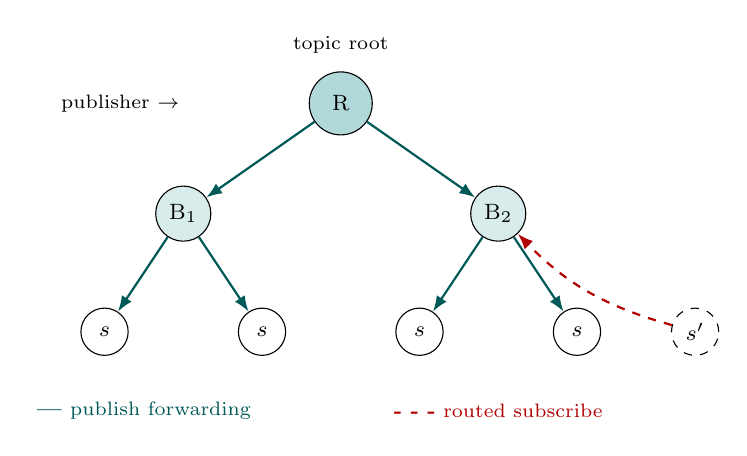
\begin{tikzpicture}[
  every node/.style={font=\footnotesize},
  root/.style={circle, draw, fill=teal!30, minimum size=8mm, inner sep=0pt},
  branch/.style={circle, draw, fill=teal!15, minimum size=7mm, inner sep=0pt},
  sub/.style={circle, draw, minimum size=6mm, inner sep=0pt},
  newsub/.style={circle, draw, dashed, minimum size=6mm, inner sep=0pt},
  pubarr/.style={-{Latex[length=2mm]}, thick, color=teal!70!black},
  subarr/.style={-{Latex[length=2mm]}, thick, dashed, color=red!70!black},
]
% Root
\node[root] (R) at (0, 2.4) {R};
\node[above=1mm of R, font=\scriptsize] {topic root};

% Branches
\node[branch] (B1) at (-2.0, 1.0) {B$_1$};
\node[branch] (B2) at (2.0, 1.0) {B$_2$};

% Subscribers under B1
\node[sub] (s1) at (-3.0, -0.5) {$s$};
\node[sub] (s2) at (-1.0, -0.5) {$s$};

% Subscribers under B2
\node[sub] (s3) at (1.0, -0.5) {$s$};
\node[sub] (s4) at (3.0, -0.5) {$s$};

% New subscriber attaching
\node[newsub] (sn) at (4.5, -0.5) {$s'$};

% Publish forwarding (solid)
\draw[pubarr] (R) -- (B1);
\draw[pubarr] (R) -- (B2);
\draw[pubarr] (B1) -- (s1);
\draw[pubarr] (B1) -- (s2);
\draw[pubarr] (B2) -- (s3);
\draw[pubarr] (B2) -- (s4);

% New subscriber routes upward; intercepted at B2
\draw[subarr] (sn) to[bend left=15] (B2);

% Publisher icon
\node[font=\scriptsize, draw=none] at (-2.8, 2.4) {publisher $\to$};

% Legend
\node[font=\scriptsize, color=teal!70!black] at (-2.5, -1.5) {\textbf{---} publish forwarding};
\node[font=\scriptsize, color=red!70!black]  at ( 2.0, -1.5) {\textbf{- - -} routed subscribe};
\end{tikzpicture}
\caption{Axon-tree formation. A new subscriber $s'$ issues a routed
\textsc{subscribe} toward $\mathrm{topicId}$ (red dashed); the first
live axon role on the path (here, $B_2$) intercepts and adopts it.
Publishes flow from the root R through the branches to all subscribers
(teal solid). Tree healing under churn is the same mechanism: a
subscriber whose parent dies re-issues its subscribe, attaches to
whichever live ancestor is now closest, and continues receiving
publishes after one refresh interval.}
\label{fig:axon}
\end{figure}

\paragraph{Branching: external-peer batch adoption.}
When an axon's direct child count exceeds $\mathrm{maxDirectSubs}$, it
selects a synaptome peer (\emph{external} to its current children) as a
new sub-axon, partitions its current children by XOR proximity to the
sub-axon, and ships the relevant batch in a single
\textsc{adopt\_subscribers} message. Two invariants prevent runaway
recursion: branches always go to peers \emph{outside} the current
subtree, and the new branch's capacity is checked before adoption. Tree
depth grows as $O(\log_{C} S)$ in subscribers $S$ given capacity $C$.

\paragraph{Self-healing: re-subscribe as liveness.}
Every axon role re-issues its subscribe on a fixed refresh interval
(default $10$\,s). The walk lands on whichever live axon is closest to
$\mathrm{topicId}$ \emph{now}. If the parent died, the re-subscribe
attaches to a different live ancestor. If the tree was reorganized,
the change is invisible to the subscriber. \emph{The re-subscribe is
the liveness check} --- there is no separate ping, no parent tracking,
no gossip. The protocol exploits the same mechanism that builds the
tree to repair it.

\paragraph{Temporal pub/sub.}
A subscribe is not just ``send me future messages.'' It is ``send me
every message I have not already seen.'' Each subscribe carries a
$\mathrm{lastSeenTs}$ --- the highest publish timestamp the subscriber
has observed. Every relay maintains a bounded ring buffer (default
$100$ messages per topic). On subscribe arrival, the relay replays
filtered cache entries with $\mathrm{publishTs} > \mathrm{lastSeenTs}$
as a single batched message before forwarding the subscribe upstream.
Healing and replay are the \emph{same} mechanism: a subscriber
attaching to a new branch after parent death receives both the
attachment and any messages that elapsed during the gap.

% ═════════════════════════════════════════════════════════════════════════════
\section{The Geographic DHT (\GDHT)}
\label{sec:gdht}

The Geographic DHT (\GDHT) is the second protocol contribution of this
paper. It is a simple structural extension of Kademlia that gives the
overlay an awareness of physical locality without changing the routing
algorithm itself. \GDHT serves throughout the rest of the paper as the
geographically-aware substrate on which \nhone's learning is layered,
and as the comparative baseline against which \nhone is measured.

\subsection{Construction}
\label{sec:gdht-construction}

Every node identifier is composed by concatenating an S2 cell prefix
with a public-key hash:
\begin{equation}
\mathrm{nodeId} = \underbrace{\mathrm{S2cell}_{8}}_{\text{8 bits}} \;\Vert\; \underbrace{H(\mathrm{publicKey})}_{\text{56 bits}}
\label{eq:gdht-id}
\end{equation}
The S2 library~\cite{s2geometry} maps every point on Earth to a $64$-bit
cell ID along a Hilbert space-filling curve projected through six cube
faces. The top $8$ bits encode the cube face plus a $5$-bit Hilbert
subdivision, yielding $6 \times 32 = 192$ continent-scale tiles
worldwide (typical examples: ``western North America,'' ``South-East
Asia''). The Hilbert curve property ensures that geographically
adjacent points have numerically close cell IDs: \emph{XOR distance
in identifier space approximates physical distance, for free.}

The remaining $56$ bits are the standard cryptographic hash of the
node's public key. There is no other change to Kademlia: $K$-buckets,
$\alpha$-parallel \textsc{find\_node}, and the iterative refinement
algorithm are all retained verbatim. The locality property emerges
from the ID structure alone, with no algorithmic complexity added.

\subsection{Why this matters: the back-of-the-envelope}
\label{sec:gdht-math}

A pure Kademlia overlay with $N = 10^6$ uniformly-distributed nodes
requires $\log_2 N \approx 20$ hops per lookup. Each hop traverses a
random pair of nodes separated on average by half the planet, with
about $100$\,ms one-way round-trip time. The naive estimate gives an
average message time of $20 \times 100 = 2$\,seconds.

\GDHT changes the calculation. Most of a typical user's traffic is
\emph{geographically local} --- social, transactional, real-time. With
the location prefix, local connections are XOR-close in identifier
space, so a regional lookup operates within a much smaller effective
network. Suppose a particular region holds $\sim\!10\,000$ nodes with
typical inter-node RTT of $\sim\!7$\,ms within a continental cell.
Then $\log_2(10\,000) \approx 13$ hops $\times\ 7$\,ms $\approx
91$\,ms for an in-region message --- more than a $20\times$ improvement
over the global Kademlia number on the same total network.

The mechanism for cross-region routing is what we call a
\emph{network of networks}: when communicating with a far-away node,
\GDHT first locates \emph{any} peer inside the destination's
geographic neighborhood, then refines locally inside that
neighborhood. The long-haul hop happens \emph{once} per lookup, not
at every step. Global lookups also benefit: at $25\,000$ nodes,
\GDHT's measured global latency is $287$\,ms versus K-DHT's
$503$\,ms (Table~\ref{tab:floor}) --- a $1.75\times$ improvement
even when no part of the lookup is regional.

\subsection{Geography is a seed, not a teacher}
\label{sec:gdht-seed}

\GDHT is \emph{not} a learning protocol. The S2 prefix does not
\emph{teach} locality --- it \emph{structures} the identifier space so
that XOR-distance routing accidentally tracks physical distance for
the dominant traffic patterns. The routing table is fixed at
insertion time and lazily repaired thereafter. This is the same
class of mechanism as Pastry's locality-preserving
join~\cite{rowstron2001pastry} or Tapestry's RTT-sorted routing
table~\cite{zhao2004tapestry}, and it shares the same limitation:
without learning, the table cannot improve as the network changes.
\nhone's contribution (\S\ref{sec:nh1}) is to layer
traffic-driven learning on top of \GDHT's structural locality.
The geography ablation in \S\ref{sec:eval-geo} confirms that the
two contributions are independent: with the \GDHT prefix removed
($\mathrm{geoBits} = 0$), \nhone still routes $8\%$ faster than
Kademlia purely from learning.

\subsection{Cooperative trust and security tradeoff}
\label{sec:gdht-trust}

The S2 prefix is \emph{self-declared}. A node can claim any prefix it
wants; the protocol does not verify the claim against any external
ground truth. This is acceptable when locality benefits are
cooperative --- well-behaved peers do not lie, and an attacker who
falsifies a prefix degrades only the locality benefit, not routing
correctness. The \emph{adversarial} consequences are real: a
coordinated set of nodes claiming the same prefix can mount a Sybil
swarm in a target cell or eclipse a regional namespace. Mitigations
(Vivaldi-style learned coordinates, geographic proof-of-work, IP-ASN
binding) are detailed in \S\ref{sec:future}. None of these are
implemented in the present \GDHT; the tradeoff between locality
benefit and identity-region disclosure is, today, a deployment
choice. A privacy-sensitive deployment may choose to spoof the
prefix, accepting reduced locality in exchange for region anonymity.

% ═════════════════════════════════════════════════════════════════════════════
\section{Evaluation}
\label{sec:eval}

This section reports four headline empirical results: \nhone at the
Dabek $3\delta$ analytical floor (\S\ref{sec:eval-floor}); the
geography-stripped ablation showing learning still wins
(\S\ref{sec:eval-geo}); heterogeneous-capacity deployment
(\S\ref{sec:eval-highway}); and pub/sub robustness including the
single-bridge Slice World partition test (\S\ref{sec:eval-slice}). All
data and the simulator that produced it are open-source~\cite{dhtsim2026}.

\subsection{Methodology}
\label{sec:eval-method}

The simulator is $\sim\!25\,000$ lines of JavaScript. Latency is computed
geometrically (great-circle distance scaled to a per-hop one-way
propagation delay plus $10$\,ms processing) rather than waited on, so
the simulation runs at full CPU speed. The implementation deliberately
\emph{abstracts} wall-clock transport, encryption, and node identity
to focus on routing dynamics; \S\ref{sec:discussion} discusses what
this abstraction misses. Five integrity invariants are enforced after
every churn event: (i)~bilateral connection-cap audit; (ii)~locality
preservation (no optimization reads another node's routing table
directly); (iii)~bounded $K$-element RPC envelopes; (iv)~per-protocol
parameter routing; (v)~geographic-prefix flow into every protocol's
node-ID construction.

The headline measurements use $25\,000$-node networks; we validate at
$5\,000$ and $50\,000$ nodes for the $3\delta$ result. Default
configuration: web-limited $100$-connection cap (browser-class), $50$
synaptome cap, $K=20$, $\alpha = 3$, $500$ lookups per test cell,
omniscient initialization (every protocol seeded with its theoretically
optimal $K$-closest neighbors) to isolate routing-algorithm contribution
from bootstrap variance. Where canonical initialization is used --- every
protocol forced to start from identical $K$-closest XOR routing tables
--- we say so explicitly.

\subsection{Headline: \nhone at the Dabek $3\delta$ floor}
\label{sec:eval-floor}

The Dabek bound (Eq.~\ref{eq:dabek}) requires a measured value of
$\delta$, the median pairwise one-way internet latency for the
population under test. We compute $\delta$ at the start of every
benchmark sweep by sampling $10\,000$ random node pairs and taking the
median of $\mathrm{messageLatency}(a, b)$ for each. This is independent
of any protocol and is therefore a property of the network, not of the
DHT. Table~\ref{tab:floor} reports $\delta$ together with each
protocol's measured global-lookup latency at three network sizes.

\begin{table*}[t]
\centering
\caption{Global-lookup latency (ms) versus the $3\delta$ analytical floor.
The parenthesized value is multiplicative overhead over the floor.
$\delta$ is the median pairwise one-way latency for that population, sampled per sweep over $10\,000$ random node pairs.}
\label{tab:floor}
\small
\begin{tabular}{@{}lrrrrrr@{}}
\toprule
$N$ & $\delta$ (ms) & $3\delta$ floor (ms) & K-DHT & G-DHT & \NXseventeen & \nhone \\
\midrule
$5\,000$  & $67.9$ & $204$ & $410$\ ($2.01\times$) & $268$\ ($1.32\times$) & $\mathbf{215}$\ ($\mathbf{1.06\times}$) & $240$\ ($1.18\times$) \\
$25\,000$ & $68.0$ & $204$ & $503$\ ($2.46\times$) & $287$\ ($1.41\times$) & $\mathbf{241}$\ ($\mathbf{1.18\times}$) & $254$\ ($1.25\times$) \\
$50\,000$ & $68.9$ & $207$ & $548$\ ($2.65\times$) & $291$\ ($1.41\times$) & $\mathbf{243}$\ ($\mathbf{1.18\times}$) & $264$\ ($1.28\times$) \\
\bottomrule
\end{tabular}
\end{table*}

The result has three parts.
Figure~\ref{fig:floor} plots the protocol curves against the analytical
reference line.

\begin{figure}[t]
\centering
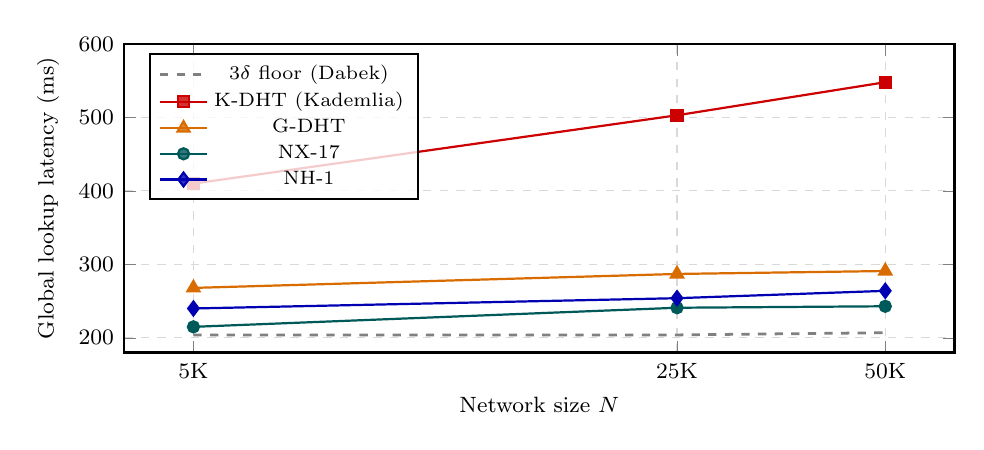
\begin{tikzpicture}
\begin{axis}[
  width=\columnwidth,
  height=5.5cm,
  xlabel={Network size $N$},
  ylabel={Global lookup latency (ms)},
  xmode=log,
  log basis x={10},
  legend pos=north west,
  legend style={font=\scriptsize, fill=white, fill opacity=0.8, draw opacity=1, text opacity=1, row sep=-1pt},
  xtick={5000, 25000, 50000},
  xticklabels={5K, 25K, 50K},
  ytick={200, 300, 400, 500, 600},
  ymin=180, ymax=600,
  grid=major,
  grid style={dashed, gray!30},
  font=\footnotesize,
  thick,
]
\addplot[dashed, color=gray, mark=none, line width=1pt] coordinates {(5000, 204) (25000, 204) (50000, 207)};
\addlegendentry{$3\delta$ floor (Dabek)}
\addplot[color=red!80!black, mark=square*, mark size=2pt] coordinates {(5000, 410) (25000, 503) (50000, 548)};
\addlegendentry{K-DHT (Kademlia)}
\addplot[color=orange!85!black, mark=triangle*, mark size=2.5pt] coordinates {(5000, 268) (25000, 287) (50000, 291)};
\addlegendentry{G-DHT}
\addplot[color=teal!70!black, mark=*, mark size=2pt] coordinates {(5000, 215) (25000, 241) (50000, 243)};
\addlegendentry{NX-17}
\addplot[color=blue!70!black, mark=diamond*, mark size=2.5pt] coordinates {(5000, 240) (25000, 254) (50000, 264)};
\addlegendentry{NH-1}
\end{axis}
\end{tikzpicture}
\caption{Global-lookup latency vs network size, plotted against the
Dabek $3\delta$ analytical floor (gray dashed). \NXseventeen plateaus at
$1.18\times$ the floor at $25\,000$ and $50\,000$ nodes; \nhone at
$1.28\times$. Kademlia worsens from $2.01\times$ to $2.65\times$ over
the same range. The floor itself is essentially flat ($\delta$ is a
property of the network, not of $N$).}
\label{fig:floor}
\end{figure}

\paragraph{\nhone's predecessor plateaus at the floor.}
\NXseventeen sits at $1.18\times$ the $3\delta$ floor at both $25\,000$
and $50\,000$ nodes --- only $36$\,ms above the analytical lower bound
for any recursive $O(\log N)$ DHT. Within the geometric-series
decomposition of Eq.~\ref{eq:dabek}, the residual $18\%$ overhead has
a clean structural explanation: \NXseventeen averages $4.5$ hops where
a Dabek-ideal protocol would take $\sim\!3$. Each ``extra'' hop costs
$\sim\!\delta/2 \approx 34$\,ms --- exactly the geometric tail Dabek's
series predicts.

\paragraph{Kademlia worsens with $N$.}
K-DHT goes from $2.01\times$ at $5\,000$ to $2.65\times$ at $50\,000$.
The log-$N$ hop tax compounds: more hops, each at full pairwise
latency, each contributing fully to the total. Kademlia is locality-blind
by construction.

\paragraph{$\delta$ is uncannily close to Dabek's measurement.}
Our simulator's median pairwise one-way latency is $67$--$69$\,ms across
network sizes. Dabek \emph{et~al.}'s King-dataset measurement reports a
median of $67$\,ms~\cite{dabek2004designing}. The simulator's geometric
latency model and Dabek's wide-area Internet measurements agree
quantitatively --- which validates the bound's transferability from
the King dataset to our population-distributed simulator.

\subsection{Learning beats locality without geography}
\label{sec:eval-geo}

A skeptical reader of \S\ref{sec:eval-floor} might suspect the
geographic prefix is doing all the work. To answer this, we strip
the prefix ($\mathrm{geoBits} = 0$, identifiers are random hashes of
public keys with no geographic structure) and re-run the comparison
with canonical initialization at $25\,000$ nodes (Table~\ref{tab:geo}).

\begin{table}[t]
\centering
\caption{Geography ablation. Global-lookup latency in milliseconds at
$25\,000$ nodes, canonical initialization. ``Improvement vs.\ Kademlia''
isolates the contribution of learning under no-geography conditions.}
\label{tab:geo}
\small
\setlength{\tabcolsep}{4pt}
\begin{tabular}{@{}lrrr@{}}
\toprule
\textbf{Protocol} & \textbf{geoBits=0} & \textbf{geoBits=8} & \textbf{Improvement} \\
\midrule
K-DHT & $506$ & $508$ & --- (baseline) \\
\GDHT & $780$\textsuperscript{$\dagger$} & $284$ & --- (geo is mechanism) \\
\NXseventeen & $\mathbf{376}$ & $\mathbf{241}$ & $\mathbf{-26\%}$ from learning \\
\nhone & $467$ & $269$ & $-8\%$ from learning \\
\bottomrule
\multicolumn{4}{l}{\footnotesize\textsuperscript{$\dagger$}\GDHT's
$\mathrm{geoBits} = 0$ result reflects its $\mathrm{noProgressLimit} = 3$} \\
\multicolumn{4}{l}{\footnotesize lookup-tuning choice; with no geographic
gradient the extra} \\
\multicolumn{4}{l}{\footnotesize ``no progress'' rounds are wasted overhead.}
\end{tabular}
\end{table}

The headline: \emph{with no geographic information whatsoever},
\NXseventeen routes lookups $26\%$ faster than Kademlia and \nhone
routes them $8\%$ faster --- purely from LTP-driven path reinforcement.
Add the S2 prefix back in and the gap widens further. This is the
cleanest possible ``learning helps'' claim: every confound (bootstrap
strategy, identifier structure, geographic prefix) is controlled, and
the routing/learning algorithm still wins. Geography helps; geography
is not necessary.

\subsection{Heterogeneous capacity (highway\%)}
\label{sec:eval-highway}

Real peer-to-peer networks are heterogeneous. We sweep the fraction of
server-class nodes from $0$ to $100\%$ at $25\,000$ total nodes;
Table~\ref{tab:highway} reports five points.

\begin{table}[t]
\centering
\caption{Latency under mixed-capacity deployment. ``Highway~\%'' is the
fraction of server-class peers (synaptome cap raised from $50$ to $256$,
unlimited inbound). The remaining peers stay browser-class.}
\label{tab:highway}
\small
\setlength{\tabcolsep}{6pt}
\begin{tabular}{@{}rrrr@{}}
\toprule
\textbf{Highway \%} & \textbf{Global ms} & \textbf{$500$\,km ms} & \textbf{$2000$\,km ms} \\
\midrule
$0$ (all browser) & $263$ & $96$ & $123$ \\
$5$ & $248$ & $81$ & $108$ \\
\textbf{$15$ (knee)} & $\mathbf{223}$ & $\mathbf{69}$ & $\mathbf{98}$ \\
$30$ & $223$ & $60$ & $83$ \\
$50$ & $212$ & $55$ & $84$ \\
$100$ (all server) & $206$ & $45$ & $74$ \\
\bottomrule
\end{tabular}
\end{table}

The result: $15\%$ server-class nodes captures $70\%$ of the
available improvement over the all-browser baseline ($263 \to 223$ vs
$263 \to 206$ for $100\%$ server). Beyond $15\%$, additional server
capacity yields diminishing returns. This is a deployment-realistic
finding: a real network does not need a uniform server fleet.

\subsection{Pub/sub robustness and partition healing}
\label{sec:eval-slice}

\paragraph{Steady-state delivery.} At $25\,000$ nodes with $79$ topic
groups of $32$ subscribers each, \nhone delivers $100.0\%$ of publishes
in steady state. Under $5\%$ instantaneous churn, immediate delivery
falls to $99.9\%$ and recovers to $100.0\%$ after three refresh
intervals. There are no orphans, no dead children, and the
publisher-subscriber view overlap (subscribers' top-$K$ vs publisher's
top-$K$) remains at $99.5\%$.

\paragraph{Graceful degradation under sustained churn.} Continuous
churn at $1\%$ of alive nodes per $5$ ticks, with three refresh passes
between kills, produces a smooth degradation curve: $98.7\%$ delivered
at $5\%$ cumulative churn, $91.2\%$ at $10\%$, $86.5\%$ at $20\%$,
$70.0\%$ at $25\%$, $52.4\%$ at $30\%$. Crucially, there is no cliff:
delivery degrades linearly with churn, indicating that the protocol
finds a steady state where new-subscriber recruitment matches
loss. The dominant residual failure mode at high churn is not broken
routing but \emph{subscribers temporarily captured at relays that have
lost their delivery path to the root} --- the failure mode the
temporal replay cache (\S\ref{sec:pubsub}) was designed to close.

\paragraph{Slice World: partition recovery from a single bridge.}
The Slice World test partitions the network into Eastern and Western
hemispheres connected through \emph{a single bridge node} placed near
Hawaii. Every cross-hemisphere edge except those incident on the
bridge is removed before the test begins. The question is not ``can
the protocol find the bridge?'' --- that is a one-shot routing
problem. The question is: \emph{given the single bridge, can the
protocol leverage repeated successful crossings to dissolve the
partition?}

\begin{table}[t]
\centering
\caption{Slice World single-bridge partition recovery. ``Slice
success~\%'' is the lookup success rate over a $500$-lookup
cross-partition workload after partition setup.}
\label{tab:slice}
\small
\begin{tabular}{@{}lrr@{}}
\toprule
\textbf{Protocol} & \textbf{Slice success~\%} & \textbf{Slice ms} \\
\midrule
K-DHT (Kademlia) & $0.0\%$ & --- (no recovery) \\
\GDHT & $4.6\%$ & $525$ (no recovery) \\
\NXseventeen & $94.8\%$ & $423$ \\
\nhone & $\mathbf{94.4\%}$ & $\mathbf{462}$ \\
\bottomrule
\end{tabular}
\end{table}

Table~\ref{tab:slice} reports the result. K-DHT achieves $0\%$
success: with no learning, the partition is permanent. \GDHT achieves
$4.6\%$: the geographic prefix happens to point a few peers at the
bridge, but no mechanism amplifies the discovery. \NXseventeen and
\nhone both achieve $\sim\!94\%$ success.

The mechanism is the bridge as \emph{seed crystal}. A diagnostic run
at $5\,000$ nodes shows the recovery directly. After a fresh partition
($0$ cross-hemisphere synapses), running just $10$ lookups yields $20$
new cross-hemisphere synapses (an average of $\sim\!3$ per
successful crossing). Hop caching (Rule~8) installs the destination
in every intermediate node along the bridge path. Triadic closure
(Rule~7) introduces direct edges between observed transit pairs.
Lateral spread propagates the new edge to the source's geographic
neighbors. By $500$ lookups, hundreds of cross-hemisphere synapses
exist; the partition has effectively dissolved. The $94\%$ aggregate
success rate is the \emph{integral} of recovery, not a snapshot of
bridge-finding. \nhone and \NXseventeen route through the partition
not by finding the bridge each time --- they \emph{dissolve} the
partition.

\subsection{Bandwidth concentration: empirical resolution}
\label{sec:eval-bandwidth}

The companion red-team analysis~\cite{nh1redteam2026} ranks
\emph{bandwidth saturation and congestion collapse} as a critical
deploy blocker (Issue~\#3). Of the four Tier~1 issues, three
(connection setup, RPC timeouts, latency jitter) are textbook
engineering problems with known mitigations. Issue~\#3 was different:
the simulator's uniform-cost-per-hop model (\S\ref{sec:eval-method})
made it \emph{architecturally unfalsifiable} whether \nhone's
adaptive routing concentrated load (the success-disaster oscillation
hypothesized by the red team) or distributed it. Until that question
was answered, every other claim about the protocol was contingent.

\paragraph{Methodology.} We instrument every routing chokepoint with
per-node send/receive counters: the \texttt{SimulatedNetwork.send}
path used by Kademlia and \GDHT, plus a parallel \texttt{\_msg(from,
to, type)} helper invoked from each conceptual wire site in \nhone
and the NX-6 lineage (NX-6 through \NXseventeen) where routing
bypasses the simulated transport via direct map access. Sites
include: each lookup-hop transition; two-hop AP probes; hop-caching
writes; lateral-spread propagation; LTP reinforcement walks;
triadic-closure introductions; bilateral bootstrap handshakes; the
2-hop neighbour scan used by \texttt{\_localCandidate} (annealing and
dead-peer replacement); pub/sub \texttt{routeMessage} forwarding; and
\texttt{sendDirect} entry. Per-cycle counters are reset after each
training session, so the captured numbers are deltas.

For each cycle we report total messages, mean / p50 / p99 / max
per-node loads, the Gini coefficient of the per-node distribution,
and counts of nodes exceeding $10\times$ and $100\times$ the cycle
mean. The $100\times$ threshold corresponds to nodes whose absolute
forwarding rate is two orders of magnitude above peers --- the
practical definition of a bandwidth-saturation hazard.

\paragraph{Headline result: distribution shape, $4 \times 4$
sweep.} Across $42$ runs spanning four protocols (\textsc{K-DHT},
\GDHT, \NXseventeen, \nhone) and four sizes ($5\mathrm{K}$,
$10\mathrm{K}$, $25\mathrm{K}$, $50\mathrm{K}$), the load
distribution diverges sharply between classical and adaptive
protocols (Table~\ref{tab:bandwidth}).

\begin{table*}[t]
\centering
\caption{Steady-state per-cycle traffic distribution at $50\,000$
nodes, $500$ lookups per cycle, $10$ training sessions. ``Hot
$>100\times$'' counts nodes processing more than $100\times$ the
network mean per cycle --- the bandwidth-saturation hazard
threshold.}
\label{tab:bandwidth}
\small
\begin{tabular}{@{}lrrrrr@{}}
\toprule
\textbf{Protocol} & \textbf{Total/cyc} & \textbf{Gini} &
\textbf{max/mean} & \textbf{Hot~$>10\times$} &
\textbf{Hot~$>100\times$} \\
\midrule
\textsc{K-DHT} & $14{,}463$ & $\mathbf{0.940}$ & $208\times$ &
$551$ & $\mathbf{56}$ \\
\GDHT          & $17{,}633$ & $\mathbf{0.932}$ & $213\times$ &
$423$ & $\mathbf{62}$ \\
\NXseventeen   & $359{,}459$ & $0.694$ & $61\times$ & $1{,}524$ &
$\mathbf{0}$ \\
\nhone         & $416{,}071$ & $0.661$ & $47\times$ & $1{,}419$ &
$\mathbf{0}$ \\
\bottomrule
\end{tabular}
\end{table*}

The hypothesis the red team raised --- \emph{that adaptive routing
concentrates more than static routing} --- is empirically
inverted. Kademlia and \GDHT develop $56$--$62$ catastrophic-bandwidth
nodes at $50\mathrm{K}$ (max/mean ratios $> 200\times$); \nhone
produces \emph{zero} such nodes at any tested scale. The classical
DHTs' Gini coefficient grows monotonically with $N$ ($0.876
\rightarrow 0.940$ from $5\mathrm{K}$ to $50\mathrm{K}$), while
\nhone's grows much more slowly ($0.549 \rightarrow 0.661$).

\paragraph{Long-run stability.} A $50$-session run at $50\mathrm{K}$
nodes confirms the steady state is genuinely steady. Gini holds in
$[0.657, 0.668]$ across all $50$ cycles (standard deviation
$0.0025$); first-half versus second-half drift is $+0.002$. Hot
$>10\times$ count holds in $[1378, 1453]$; hot $>100\times$ count is
zero throughout. Average hops trend gently downward
($5.55 \rightarrow 5.27$): the network keeps learning without
disturbing the load profile.

\paragraph{Decomposition of the $25\times$ volume tax.} \nhone's
total traffic is $25$--$30\times$ Kademlia's. Per-type
instrumentation isolates the cost. At $50\mathrm{K}$:

\begin{table}[t]
\centering
\caption{Per-type traffic decomposition for \nhone at
$50\,000$ nodes, $500$ lookups per cycle. Counts are total
sender-plus-receiver bumps; wire-message count is half. Routing-hop
\texttt{find\_node} traffic is $1.3\%$ of all traffic; the remaining
$98.7\%$ is learning side-effects.}
\label{tab:bandwidth-types}
\small
\begin{tabular}{@{}lrr@{}}
\toprule
\textbf{Message type} & \textbf{Count/cyc} & \textbf{\%} \\
\midrule
\texttt{local\_probe} (2-hop annealing scan) & $370{,}566$ &
$\mathbf{89.1\%}$ \\
\texttt{lookahead\_probe} (two-hop AP) & $20{,}525$ & $4.9\%$ \\
\texttt{lateral\_spread} & $7{,}474$ & $1.8\%$ \\
\texttt{hop\_cache\_lateral} & $6{,}404$ & $1.5\%$ \\
\texttt{find\_node} (actual routing hop) & $5{,}538$ & $1.3\%$ \\
\texttt{hop\_cache} & $3{,}737$ & $0.9\%$ \\
\texttt{reinforce} (LTP feedback) & $1{,}823$ & $0.4\%$ \\
\bottomrule
\end{tabular}
\end{table}

A single mechanism --- the 2-hop neighbour scan in
\texttt{\_localCandidate}, used by simulated annealing and dead-peer
replacement --- accounts for $89\%$ of \nhone's wire traffic. We
introduce a parameter \texttt{annealRateScale} that multiplies the
per-hop annealing trigger probability without disturbing the
temperature-reheat semantics that fire on dead-peer detection
(preserving churn-recovery behaviour).

\paragraph{The rate-knee.} Sweeping
\texttt{annealRateScale} $\in \{0.05, 0.10, 0.25, 0.50, 1.00\}$ at
$50\mathrm{K}$ nodes (Table~\ref{tab:rate-knee}), \texttt{local\_probe}
scales linearly with the rate (perfect $10\times$ reduction at rate
$0.10$). Routing quality is unchanged across the entire range: hops
$5.48$--$5.54$, time $268$--$271\,\mathrm{ms}$, success $100\%$. The
knee is at rate $\approx 0.10$ --- the setting at which absolute
hot-node count drops to its minimum ($575$ at rate $0.10$ versus
$1{,}428$ at rate $1.00$ and $852$ at rate $0.05$).

\begin{table*}[t]
\centering
\caption{\texttt{annealRateScale} knee for \nhone at $50\,000$ nodes.
Routing quality (hops, time, success) is unchanged across the entire
range.}
\label{tab:rate-knee}
\small
\begin{tabular}{@{}rrrrrr@{}}
\toprule
\textbf{rate} & \textbf{Total/cyc} & \textbf{local\_probe} &
\textbf{Gini} & \textbf{Hot~$>10\times$} & \textbf{vs default} \\
\midrule
$0.05$ & $63{,}847$ & $18{,}224$ & $0.866$ & $852$ & $6.5\times$ cut \\
$\mathbf{0.10}$ & $\mathbf{82{,}650}$ & $\mathbf{36{,}989}$ &
$\mathbf{0.834}$ & $\mathbf{575}$ & $\mathbf{5.0\times}$ \textbf{cut} \\
$0.25$ & $137{,}363$ & $92{,}453$ & $0.770$ & $735$ & $3.0\times$ cut \\
$0.50$ & $232{,}749$ & $187{,}366$ & $0.713$ & $1{,}215$ &
$1.8\times$ cut \\
$1.00$ & $414{,}929$ & $369{,}552$ & $0.661$ & $1{,}428$ & (default) \\
\bottomrule
\end{tabular}
\end{table*}

\paragraph{Robustness under churn.} Under $5\%$ per-cycle node
turnover at $25\,000$ nodes (Table~\ref{tab:bandwidth-churn}),
throttled \nhone holds $100\%$ routing success with
Gini~$0.79$ --- still strictly better than Kademlia's $0.92$ ---
and zero hot $>100\times$ nodes. Both classical protocols develop
$7$ catastrophic-bandwidth nodes under the same churn load. The
T\_REHEAT mechanism still fires on dead-peer detection regardless of
the base annealing rate, so churn-recovery is uncompromised by the
throttle: \nhone's churn-induced Gini increase ($+0.012$) is the
smallest of any protocol tested.

\begin{table*}[t]
\centering
\caption{Steady-state distribution at $25\,000$ nodes with $5\%$
per-cycle churn.}
\label{tab:bandwidth-churn}
\small
\begin{tabular}{@{}lrrrr@{}}
\toprule
\textbf{Protocol} & \textbf{Total/cyc} & \textbf{Gini} &
\textbf{Hot~$>100\times$} & \textbf{Success} \\
\midrule
\textsc{K-DHT} & $12{,}725$ & $0.919$ & $\mathbf{7}$ & $100\%$ \\
\GDHT & $15{,}817$ & $0.910$ & $\mathbf{7}$ & $99.9\%$ \\
\NXseventeen (default) & $496{,}256$ & $0.678$ & $0$ & $100\%$ \\
\nhone (default) & $356{,}358$ & $0.654$ & $0$ & $100\%$ \\
\textbf{\nhone (throttled)} & $\mathbf{71{,}695}$ & $\mathbf{0.786}$ &
$\mathbf{0}$ & $\mathbf{100\%}$ \\
\bottomrule
\end{tabular}
\end{table*}

\paragraph{Reclassification of red-team Issue~\#3.} The foundational
concentration question is empirically resolved: \nhone distributes
load broadly and stably; classical DHTs concentrate it
catastrophically at scale. The $25\times$ volume tax of full
annealing is a single tunable parameter with a clean knee and zero
impact on routing quality. The remaining bandwidth-saturation concern
--- a popular pub/sub topic's root saturating from publish volume
under Zipf workloads --- is a bounded sub-problem whose mitigation
(hot-axon-root migration plus MaxDisjoint replication,
\S\ref{sec:future}) was already specified by the red team. The
deploy-blocker framing of the broader issue is retired.

% ═════════════════════════════════════════════════════════════════════════════
\section{Discussion and Limitations}
\label{sec:discussion}

\subsection{What \nhone adds beyond predecessors}

\paragraph{Versus Pastry and Tapestry.} Both put locality in the
routing table; both populate routing-table slots with closest-by-RTT
peers at insertion time. \nhone retains this property dynamically
through AP scoring and extends it: routing tables \emph{evolve} via
LTP, hop caching, triadic closure, and lateral spread, rather than
being set once at insertion and lazily repaired.

\paragraph{Versus Coral DSHT.} Coral builds nested RTT clusters
explicitly. \nhone consolidates the cluster hierarchy into a single
vitality-scored set: the high-vitality core plays the local-cluster
role, mid-vitality entries cover wider strata, and low-vitality peers
serve as candidate replacements during annealing. The structural
choice is opposite (one flat table vs.\ multiple nested) but the goal
--- latency-aware routing --- is shared.

\paragraph{Versus SCRIBE on Pastry.} \nhone integrates pub/sub directly
into the protocol rather than layering it on top. The mechanism
(routed subscribe + reverse-path forwarding) is identical to SCRIBE; the
difference is that \nhone's axon trees adapt under churn through routed
re-subscribe alone, with no replication, no gossip, and no parent
tracking. This is structurally simpler and (per
\S\ref{sec:eval-slice}) measurably effective.

\subsection{Measurement limitations}

\paragraph{Warmup dependency.} \nhone needs $\sim\!5\,000$ lookups
before the synaptome converges to its trained asymptote. The first
minute of deployment is suboptimal. We address this in
\S\ref{sec:eval-method} via warmup, but a freshly bootstrapped real
network would not have this luxury.

\paragraph{Synaptome cap of $50$.} A deliberate cross-browser WebRTC
target (Safari measured at $\sim\!95$, Firefox at $\sim\!190$, Node.js
at $\sim\!200$). Server deployments could reasonably use $200$--$500$.
The cap directly constrains the asymptote of LTP-driven specialization
and is therefore an architectural limit, not a tuning knob.

\paragraph{Locality is structural, not learned.} Without the S2 prefix,
the AP scoring's $\frac{1}{2}^{(\ell/100)}$ latency penalty is in
principle sufficient to discover locality from scratch, but our warmup
budget is too small to do so reliably (\S\ref{sec:eval-geo} shows the
$\mathrm{geoBits} = 0$ regional latency degrading by $360\%$). Future
work (\S\ref{sec:future}) replaces the structural prefix with a
Vivaldi-style learned coordinate.

\paragraph{Methodology gaps.} The evaluation uses uniform-rate lookups
on uniformly distributed targets, and uniform churn. Real workloads
are Zipf in publish rate (a few hot topics dominate) and burst-y in
churn (peak-hour patterns). Our simulator does not yet stress these.

\subsection{Red-team summary: what the simulator does not model}
\label{sec:redteam}

A companion red-team analysis~\cite{nh1redteam2026} catalogues thirteen
deployment-relevant gaps, ranked by deploy-blocker status, severity,
and time-to-fix. We summarize the four critical items because the
properties claimed in \S\ref{sec:eval} cannot be verified in production
until they are addressed:

\paragraph{Connection-setup friction.} The simulator treats new
synapses as immediately usable. Real WebRTC requires ICE + STUN/TURN
+ DTLS, taking $1.5$--$3$\,s per new synapse under typical NAT
conditions. \nhone's most important behavioral results
(Slice World re-stitching, annealing replacement, hop-caching
cascade) all depend on synapses becoming usable rapidly. Production
recovery times will be substantially worse than simulator measurements
suggest until \texttt{CONNECTION\_SETUP\_MS} is modeled.

\paragraph{RPC timeouts and asynchronous black holes.} The simulator
detects dead nodes instantaneously. Real RPCs to silently-dropped
nodes stall for multi-second timeout windows during which messages
are lost. The $100\%$ pub/sub recovery under $5\%$ churn measurement
assumes instant detection; a production-realistic figure would model
\texttt{RPC\_TIMEOUT\_MS} and asymmetric reply paths.

\paragraph{Bandwidth saturation.} \emph{Reclassified
following \S\ref{sec:eval-bandwidth}.} The hypothesis that AP
scoring concentrates load on overloaded nodes is empirically
falsified at the scales we measure: \nhone produces zero
$>100\times$-mean nodes at any tested size while Kademlia produces
$56$ at $50\mathrm{K}$ (Table~\ref{tab:bandwidth}). The residual
concern is the Zipf-distributed pub/sub case --- a single popular
topic's root saturating from publish volume rather than from routing
traffic. This is bounded sub-problem; mitigation by hot-axon-root
migration (Makris~\emph{et~al.}~\cite{makris2017novel} DFE pattern)
plus MaxDisjoint topic replication
(Harvesf-Blough~\cite{harvesf2007design}) is sketched
in \S\ref{sec:future}.

\paragraph{Latency jitter.} Real RTTs fluctuate $\pm 30\%$ from
bufferbloat, asymmetric paths, and queuing. Our distance-derived
latency is monotone and clean. The LTP exponential moving average has
an easy job in the simulator; high-frequency noise could prematurely
decay good synapses or promote lucky-but-unstable ones.

\paragraph{Bottom line.} The brain is production-ready. The body
is not --- but the body is now a \emph{measurable, scopeable} problem
rather than a tangle of interacting mechanisms.
\S\ref{sec:future} sketches the path forward; the open simulator
becomes the lab bench for the next iteration.

% ═════════════════════════════════════════════════════════════════════════════
\section{Implementation Architecture: A Two-Layer API}
\label{sec:architecture}

A working DHT has two interfaces, not one. The application above
wants to publish, subscribe, and look things up; the network below
wants to open a channel, send a message, and notice when a peer
goes silent. The protocol is the thing in between. \nhone is
structured so the protocol code is genuinely between those two
layers --- neither the application nor the network is hardwired
into the routing logic --- which is what makes the same body of
code reusable in both the simulator and the deployed system.

\subsection{The DHT contract --- application-facing}

The application sees one running node. The contract is small:
eight verbs covering lifecycle, operations, and observability.
\texttt{start} / \texttt{stop} bring the node up and down;
\texttt{join(sponsor)} / \texttt{leave} add to and depart from the
network. \texttt{lookup(targetKey)} walks the routing layer toward
a key; \texttt{subscribe} / \texttt{unsubscribe} / \texttt{publish}
ride on the axonal-tree primitive. \texttt{getNodeId},
\texttt{getSynaptome}, \texttt{getMetrics}, and \texttt{onEvent}
are the read-only observability surface.

The forbidden methods are as instructive as the present ones.
There is no method that enumerates ``all nodes,'' no method that
takes a peer-id and returns that peer's state, no method that lets
the application mutate the routing table. A DHT instance is
responsible for one node's view of the network; the simulator's
Engine creates many DHT instances and orchestrates them, but that
orchestration is a simulator concern --- it does not appear in the
contract.

\subsection{The Transport contract --- network-facing}

One Transport instance per running node; the protocol calls into
it. Twelve methods in four bands:

\begin{itemize}\itemsep2pt
\item \textbf{Lifecycle} (\texttt{start}, \texttt{stop},
  \texttt{getLocalNodeId}).
\item \textbf{Channel pool} (\texttt{openConnection},
  \texttt{closeConnection}, \texttt{isConnected}). This maps
  directly onto synaptome semantics: admit-to-synaptome corresponds
  to \texttt{openConnection}; evict corresponds to
  \texttt{closeConnection}. The bilateral connection cap is enforced
  inside the transport --- \texttt{openConnection} resolves with
  \texttt{false} if the remote refused.
\item \textbf{Messaging} (\texttt{send},
  \texttt{notify}, \texttt{onRequest}, \texttt{onNotification}).
  Two outbound primitives: request/response and fire-and-forget.
  The split matters because production transports pay round-trip
  latency for \texttt{send} but not for \texttt{notify}. \nhone
  uses \texttt{send} for the routing-tick chain
  (\texttt{lookup\_step}, \texttt{lookahead\_probe},
  \texttt{find\_closest\_set}, \texttt{local\_probe}) and
  \texttt{notify} for the LEARN side-effects (\texttt{reinforce},
  \texttt{hop\_cache}, \texttt{lateral\_spread},
  \texttt{triadic\_introduce}).
\item \textbf{Liveness} (\texttt{onPeerDied},
  \texttt{getLatency}). The transport runs a 1\,Hz ping/pong
  heartbeat on every open channel; missed pongs trigger
  \texttt{onPeerDied}. The protocol consumes \texttt{getLatency}
  for AP scoring and registers an \texttt{onPeerDied} callback
  that populates a per-node \texttt{\_deadPeers} set --- the same
  candidate-filter mechanism a production deployment uses.
\end{itemize}

The Transport contract forbids the protocol from reaching around
it: no \texttt{nodeMap.get(peerId)}, no
\texttt{peer.synaptome.values()} reads, no cross-peer field
access. Every cross-peer read happens via \texttt{send} or
\texttt{notify}.

\subsection{The simulator as deployment vehicle}

The simulator's \texttt{SimulatedNetwork} and the production
\texttt{WebRTCTransport} both implement the same Transport
contract. Twelve methods, one signature each. The simulator runs
handlers synchronously inside the call (in-process, no real RTT);
production runs them through WebRTC data channels with real RTT.
The protocol code does not switch on which transport it is using.

This is the property that lets the simulator be the deployment
vehicle. Years of \nhone benchmark numbers --- the hop counts,
latency distributions, pub/sub coverage, churn-resilience curves
in \S\ref{sec:eval} --- transfer directly to production because
the same code path runs in both worlds. A 25\,K-node parity-gate
benchmark (post-refactor v0.70.22 against the pre-refactor
v0.70.04 reference) confirmed every protocol within a 10\% target
band: \nhone within 5--8\% on hops, 1--4\% on latency; Kademlia,
\GDHT, NX-17 within 0.5--3\%. The protocol's central algorithm
--- the recursive-forwarding \texttt{lookup\_step} chain --- is
free of cross-peer state reads; the remaining
\texttt{nodeMap.get(peerId)} sites are sim-only orchestration
(node creation/destruction bookkeeping, the simulator's god's-eye
stratified bootstrap, and the local self-resolution in
\texttt{lookup}). Production replaces the bootstrap path with a
\texttt{BootstrapService} contract that handles signaling,
manifest signature verification, and QR-code pairing
out-of-band.

\paragraph{Live deployment.} As of v0.3.51 the production
Transport and BootstrapService implementations are live. The
browser-resident peer (\texttt{axona-peer}) runs at
\url{https://axona.net} on Mac, Windows, Linux, iOS, and Android
behind real-world NATs. The signaling broker
(\texttt{axona-bridge}) at \url{https://bridge.axona.net}
handles the WebRTC offer/answer exchange for browser-to-browser
channels; it carries no application traffic and any operator
can stand one up, so the rendezvous role is interchangeable.
The product name for the running network --- peer, bridge,
SDK --- is \emph{Axona}; \nhone is the routing protocol it
runs internally. The first end-user application on the live
network is \texttt{civildefense.io}, a tap-to-report incident
map whose primitives (signed posts, geographic locality,
24-hour expiry, anonymous P2P) inherit directly from this
protocol layer.

% ═════════════════════════════════════════════════════════════════════════════
\section{Future Work}
\label{sec:future}

The future-work agenda follows the red-team prioritization
\cite{nh1redteam2026} and integrates the comparative-literature
mechanisms identified in \S\ref{sec:related}.

\paragraph{Friction-realistic simulator.} Implement
\texttt{CONNECTION\_SETUP\_MS} with new synapses in a
\textsc{pending} state excluded from AP scoring until setup elapses;
\texttt{RPC\_TIMEOUT\_MS} for silently-dropped peers with
request/reply path tracing; load-dependent AP scoring; and Gaussian
jitter injection on every hop. The resulting measurements would be
\emph{production-realistic} versions of the results in \S\ref{sec:eval}.

\paragraph{Vivaldi-style learned locality.} Replace the self-declared
S2 prefix with synthetic Euclidean coordinates~\cite{dabek2004vivaldi}
that converge from observed RTTs. Learned coordinates close the
cell-eclipse gap (\S\ref{sec:gdht}) by removing the cooperative-trust
assumption: an attacker cannot falsify a coordinate that is verified
against measured RTT.

\paragraph{Byzantine pub/sub via MaxDisjoint replication.} Replicate
each axon-tree root at $d$ disjoint locations using
Harvesf-Blough's placement formula~\cite{harvesf2007design}. With
$d = 8$ replicas this delivers $90\%$ pub/sub success at $50\%$
malicious nodes per their measurement. Combined with surrogate routing
on the multicast tree, this closes the Byzantine-resistance gap without
abandoning the axonal-tree primitive.

\paragraph{Adaptive parameter tuning.} Following Ghinita and
Teo~\cite{ghinita2006adaptive}, each peer maintains a rolling estimate
of local failure rate $\mu$ and join rate $\lambda$. Annealing cooling
rate, reheat amount, and the staleness threshold for synapse eviction
all become functions of $(\mu, \lambda)$ rather than fixed constants.
A peer in a stable region anneals slowly; a peer in a high-churn
region anneals aggressively, automatically.

\paragraph{Metaplastic \nhone.} The natural endpoint of the previous
direction: expose a single QoS knob (target lookup failure rate) and
let the system self-tune underlying constants
(\texttt{decayGamma}, \texttt{INERTIA\_DURATION}, the annealing
schedule, even synaptome capacity) to hit it. This is precisely the
metaplasticity of \S\ref{sec:substrate}'s
forward-pointer: plasticity of plasticity, with the system maintaining
a homeostatic operating point rather than running on hand-picked
constants.

% ═════════════════════════════════════════════════════════════════════════════
\section{Conclusion}
\label{sec:conclusion}

We have presented \nhone, a learning-adaptive distributed hash table
that operates within $1.18$--$1.28\times$ the Dabek $3\delta$
analytical floor for recursive $O(\log N)$ routing on a $50\,000$-node
network. \nhone consolidates eighteen specialized rules and
forty-four parameters from its predecessor into twelve rules and
twelve parameters governed by a single vitality function ---
$\mathrm{weight} \times \mathrm{recency}$ --- that is a direct
application of Hebbian long-term potentiation to overlay routing.
Built-in axonal pub/sub achieves $100\%$ baseline and $100\%$
recovered delivery under $5\%$ churn through routed re-subscribe alone.
Single-bridge network partitions dissolve through cooperative
re-stitching driven by hop caching and triadic closure. Stripping the
geographic prefix shows that learning alone outperforms Kademlia by
$26\%$, demonstrating that the contribution is structural rather than
a consequence of locality engineering.

The Berkeley/Cambridge DHT lineage --- Kademlia plus Pastry plus
Tapestry plus SCRIBE --- gave us the substrate; vitality-driven
learning is the contribution. The production stack ---
\texttt{axona-peer} (the browser-resident node) and
\texttt{axona-bridge} (an interchangeable signaling broker) ---
runs the same protocol code as the simulator that produced the
numbers in \S\ref{sec:eval}. Code, data, simulator, and the
companion red-team analysis are open at
\texttt{github.com/axona-net/dht-sim}~\cite{dhtsim2026}; the live
peer and bridge sources are at \texttt{github.com/axona-net/axona-peer}
and \texttt{github.com/axona-net/axona-bridge}.

% ─────────────────────────────────────────────────────────────────────────────
\bibliographystyle{IEEEtran}
\bibliography{references}

\end{document}
